\documentclass[11pt,a4paper]{article}
\usepackage{subcaption}
% --- Базовые пакеты и шрифты ---
\usepackage[T2A]{fontenc}
\usepackage[utf8]{inputenc}
\usepackage[english, russian]{babel}
\usepackage{amsmath, amsfonts, amssymb, mathtools, stmaryrd}
\usepackage{indentfirst}
\usepackage{graphicx}
\usepackage{microtype} % Улучшает типографику

% --- Геометрия страницы ---
\usepackage{geometry}
\geometry{
    a4paper,
    total={170mm,257mm},
    left=20mm,
    top=25mm,
    bottom=20mm,
    right=20mm,
}

% --- Колонтитулы ---
\usepackage{fancyhdr}
\pagestyle{fancy}
\fancyhf{}
\fancyhead[L]{Домашнее задание по архитектурам №4}
\fancyhead[R]{Куртеев А. М. (Б01-407)}
\fancyfoot[C]{\thepage}
\renewcommand{\headrulewidth}{0.4pt}

% --- Стилизация заголовков ---
\usepackage{titlesec}
\titleformat{\section}{\large\bfseries\sffamily}{\thesection}{1em}{}

% --- Работа с графикой и TikZ ---
\usepackage{tikz}
\usepackage{tzplot}
\usepackage{pgfplots}
\usepackage{pgf-pie}
\usetikzlibrary{arrows.meta, backgrounds, positioning, fit, calc, intersections, quotes, angles, automata}
\pgfplotsset{compat=1.18}

% --- Настройка листингов кода (Modern Dark/Pastel Style) ---
\usepackage{listings}
\usepackage{xcolor}

\definecolor{base03}{HTML}{002B36}
\definecolor{base0}{HTML}{839496}
\definecolor{blue}{HTML}{268BD2}
\definecolor{cyan}{HTML}{2AA198}
\definecolor{green}{HTML}{859900}
\definecolor{magenta}{HTML}{D33682}
\definecolor{orange}{HTML}{CB4B16}

\lstdefinestyle{modernstyle}{
    backgroundcolor=\color{white},
    commentstyle=\color{gray}\itshape,
    keywordstyle=\color{blue}\bfseries,
    numberstyle=\tiny\color{base0},
    stringstyle=\color{green},
    basicstyle=\ttfamily\small,
    breakatwhitespace=false,
    breaklines=true,
    captionpos=t,
    keepspaces=true,
    numbers=left,
    numbersep=8pt,
    showspaces=false,
    showstringspaces=false,
    showtabs=false,
    tabsize=4,
    frame=single,
    rulecolor=\color{gray!30},
    xleftmargin=10pt
}
\lstset{style=modernstyle}

% --- Теоремы и определения (с рамками или отступами) ---
\newtheorem{definition}{Определение}[section]
\newtheorem{remark}{Примечание}
\newtheorem{theorem}{Теорема}[section]

% --- Пользовательские команды ---
\newcommand{\implyarrow}{\mathrel{\rotatebox[origin=c]{90}{$\Rightarrow$}}}
\DeclareMathOperator{\arccot}{arccot}

% --- Титульная часть ---
\begin{document}

\begin{center}
    \textsf{\LARGE Домашнее задание по архитектурам №4} \\
    \vspace{0.5em}
    \vspace{1.5em}
    \textbf{Куртеев Александр Михайлович (Б01-407)} \\
    \texttt{kurteev.am@phystech.edu} \\
    \vspace{1em}
    \hrule
\end{center}

\newpage

\section*{1. Описание политик и алгоритма}

\begin{itemize}
    \item \textbf{Политика замещения LRU (Least Recently Used):} Классический алгоритм вытеснения данных. Когда кэш заполняется, алгоритм удаляет строку, к которой процессор не обращался дольше всего. Исходит из принципа временной локальности: недавно использованные данные понадобятся снова, а давно неиспользуемые можно удалить.
    
    \item \textbf{Политика замещения SHiP (Signature-based Hit Predictor):} Адаптивный алгоритм, предсказывающий интервал повторного использования кэш линии на основе её сигнатуры (например хэша PC или последовательности инструкций). Обучаясь на истории обращений с помощью таблицы счетчиков (SHCT), SHiP прогнозирует, получит ли строка повторные обращения. Если нет, ей назначается далекий интервал повторного использования для скорейшего вытеснения.
    
    \item \textbf{Префетчер SPP (Signature Path Prefetcher):} Префетчер, использующий сигнатуру предыдущих доступов внутри физической страницы. SPP находит закономерности в сигнатурах и рекурсивно предсказывает следующие дельты (смещения) обращений. Алгоритм вычисляет уверенность пути и динамически меняет глубину предварительной выборки, чтобы сохранять баланс между покрытием и точностью.
\end{itemize}

\section*{2. Выбранные трассы для анализа}

Для экспериментов выбраны следующие трассы:
\begin{enumerate}
    \item \textbf{625.x264\_s-18B:} Кодирование видео. Высокая потребность в кэшировании данных и строгая локальность.
    \item \textbf{445.gobmk-17B:} Частые обращения к сложным структурам данных.
    \item \textbf{603.bwaves\_s-1080B:} Cложные вычисления, требующие больших объемов
данных и частых обращений в память. Оно нагружает кэш и может быть полезно
для анализа работы L2 кэша в условиях вычислительных интенсивных задач
\end{enumerate}

и конфигурации:
\begin{enumerate}
    \item \textbf{champsim\_lru\_no\_256s\_8w}    
    \item \textbf{champsim\_lru\_no\_512s\_8w}    
    \item \textbf{champsim\_lru\_no\_512s\_16w}   
    \item \textbf{champsim\_lru\_no\_1024s\_8w}   
    \item \textbf{champsim\_lru\_no\_1024s\_16w}  
    \item \textbf{champsim\_ship\_no\_256s\_8w}    
    \item \textbf{champsim\_ship\_no\_512s\_8w}    
    \item \textbf{champsim\_ship\_no\_512s\_16w}   
    \item \textbf{champsim\_ship\_no\_1024s\_8w}   
    \item \textbf{champsim\_ship\_no\_1024s\_16w}  
    \item \textbf{champsim\_ship\_spp\_256s\_8w}
    \item \textbf{champsim\_ship\_spp\_512s\_8w}
    \item \textbf{champsim\_ship\_spp\_512s\_16w}
    \item \textbf{champsim\_ship\_spp\_1024s\_8w}
    \item \textbf{champsim\_ship\_spp\_1024s\_16w}
\end{enumerate}

\section*{3. Методика проведения экспериментов}

Моделирование и сбор данных выполнялись при помощи потактового симулятора \texttt{ChampSim}. Ниже приведены технические характеристики системы:

\begin{itemize}
    \item \textbf{Процессор:} Intel Core i5-12450H (архитектура Alder Lake-H).
    \item \textbf{Конфигурация ядер:} 8 ядер / 12 потоков (4 высокопроизводительных P-ядра и 4 энергоэффективных E-ядра).
    \item \textbf{Тактовая частота:} Базовая частота P-ядер 2.0 ГГц с возможностью повышения до 4.4 ГГц в режиме Turbo Boost.
    \item \textbf{Параметры кэш-памяти:} L3 Smart Cache --- 12 МБ, L2 --- 7 МБ.
    \item \textbf{Оперативная память:} 16 гб DDR4.
    \item \textbf{Среда выполнения:}  Arch Linux
\end{itemize}

С целью предотвращения переполнения виртуальной памяти количество одновременно запущенных процессов симуляции было ограничено до 4 единиц с помощью утилиты \texttt{GNU Parallel}. 

\section*{4. Среднее геометрическое }

\begin{table}[h]
\centering
\begin{tabular}{|l|c|c|c|c|c|}
\hline
\textbf{Политика} & \textbf{128K} & \textbf{256K} & \textbf{512K (8w)} & \textbf{512K (16w)} & \textbf{1024K} \\ \hline
LRU & 0.6122 & 0.6343 & 0.6378 & 0.6382 & 0.6398 \\ \hline
SHIP & 0.1436 & 0.2612 & 0.3815 & 0.2682 & 0.3852 \\ \hline
SHIP+SPP & 0.1949 & 0.2644 & 0.3406 & 0.2687 & 0.3463 \\ \hline
\end{tabular}
\caption{Геометрическое среднее L2 Hit Rate по всем трассам}
\label{tab:geomean_hit_rate}
\end{table}

\section*{5. График зависимостей L2\_Hit\_Rate от размера кэша}

\begin{figure}[h!]
    \centering
     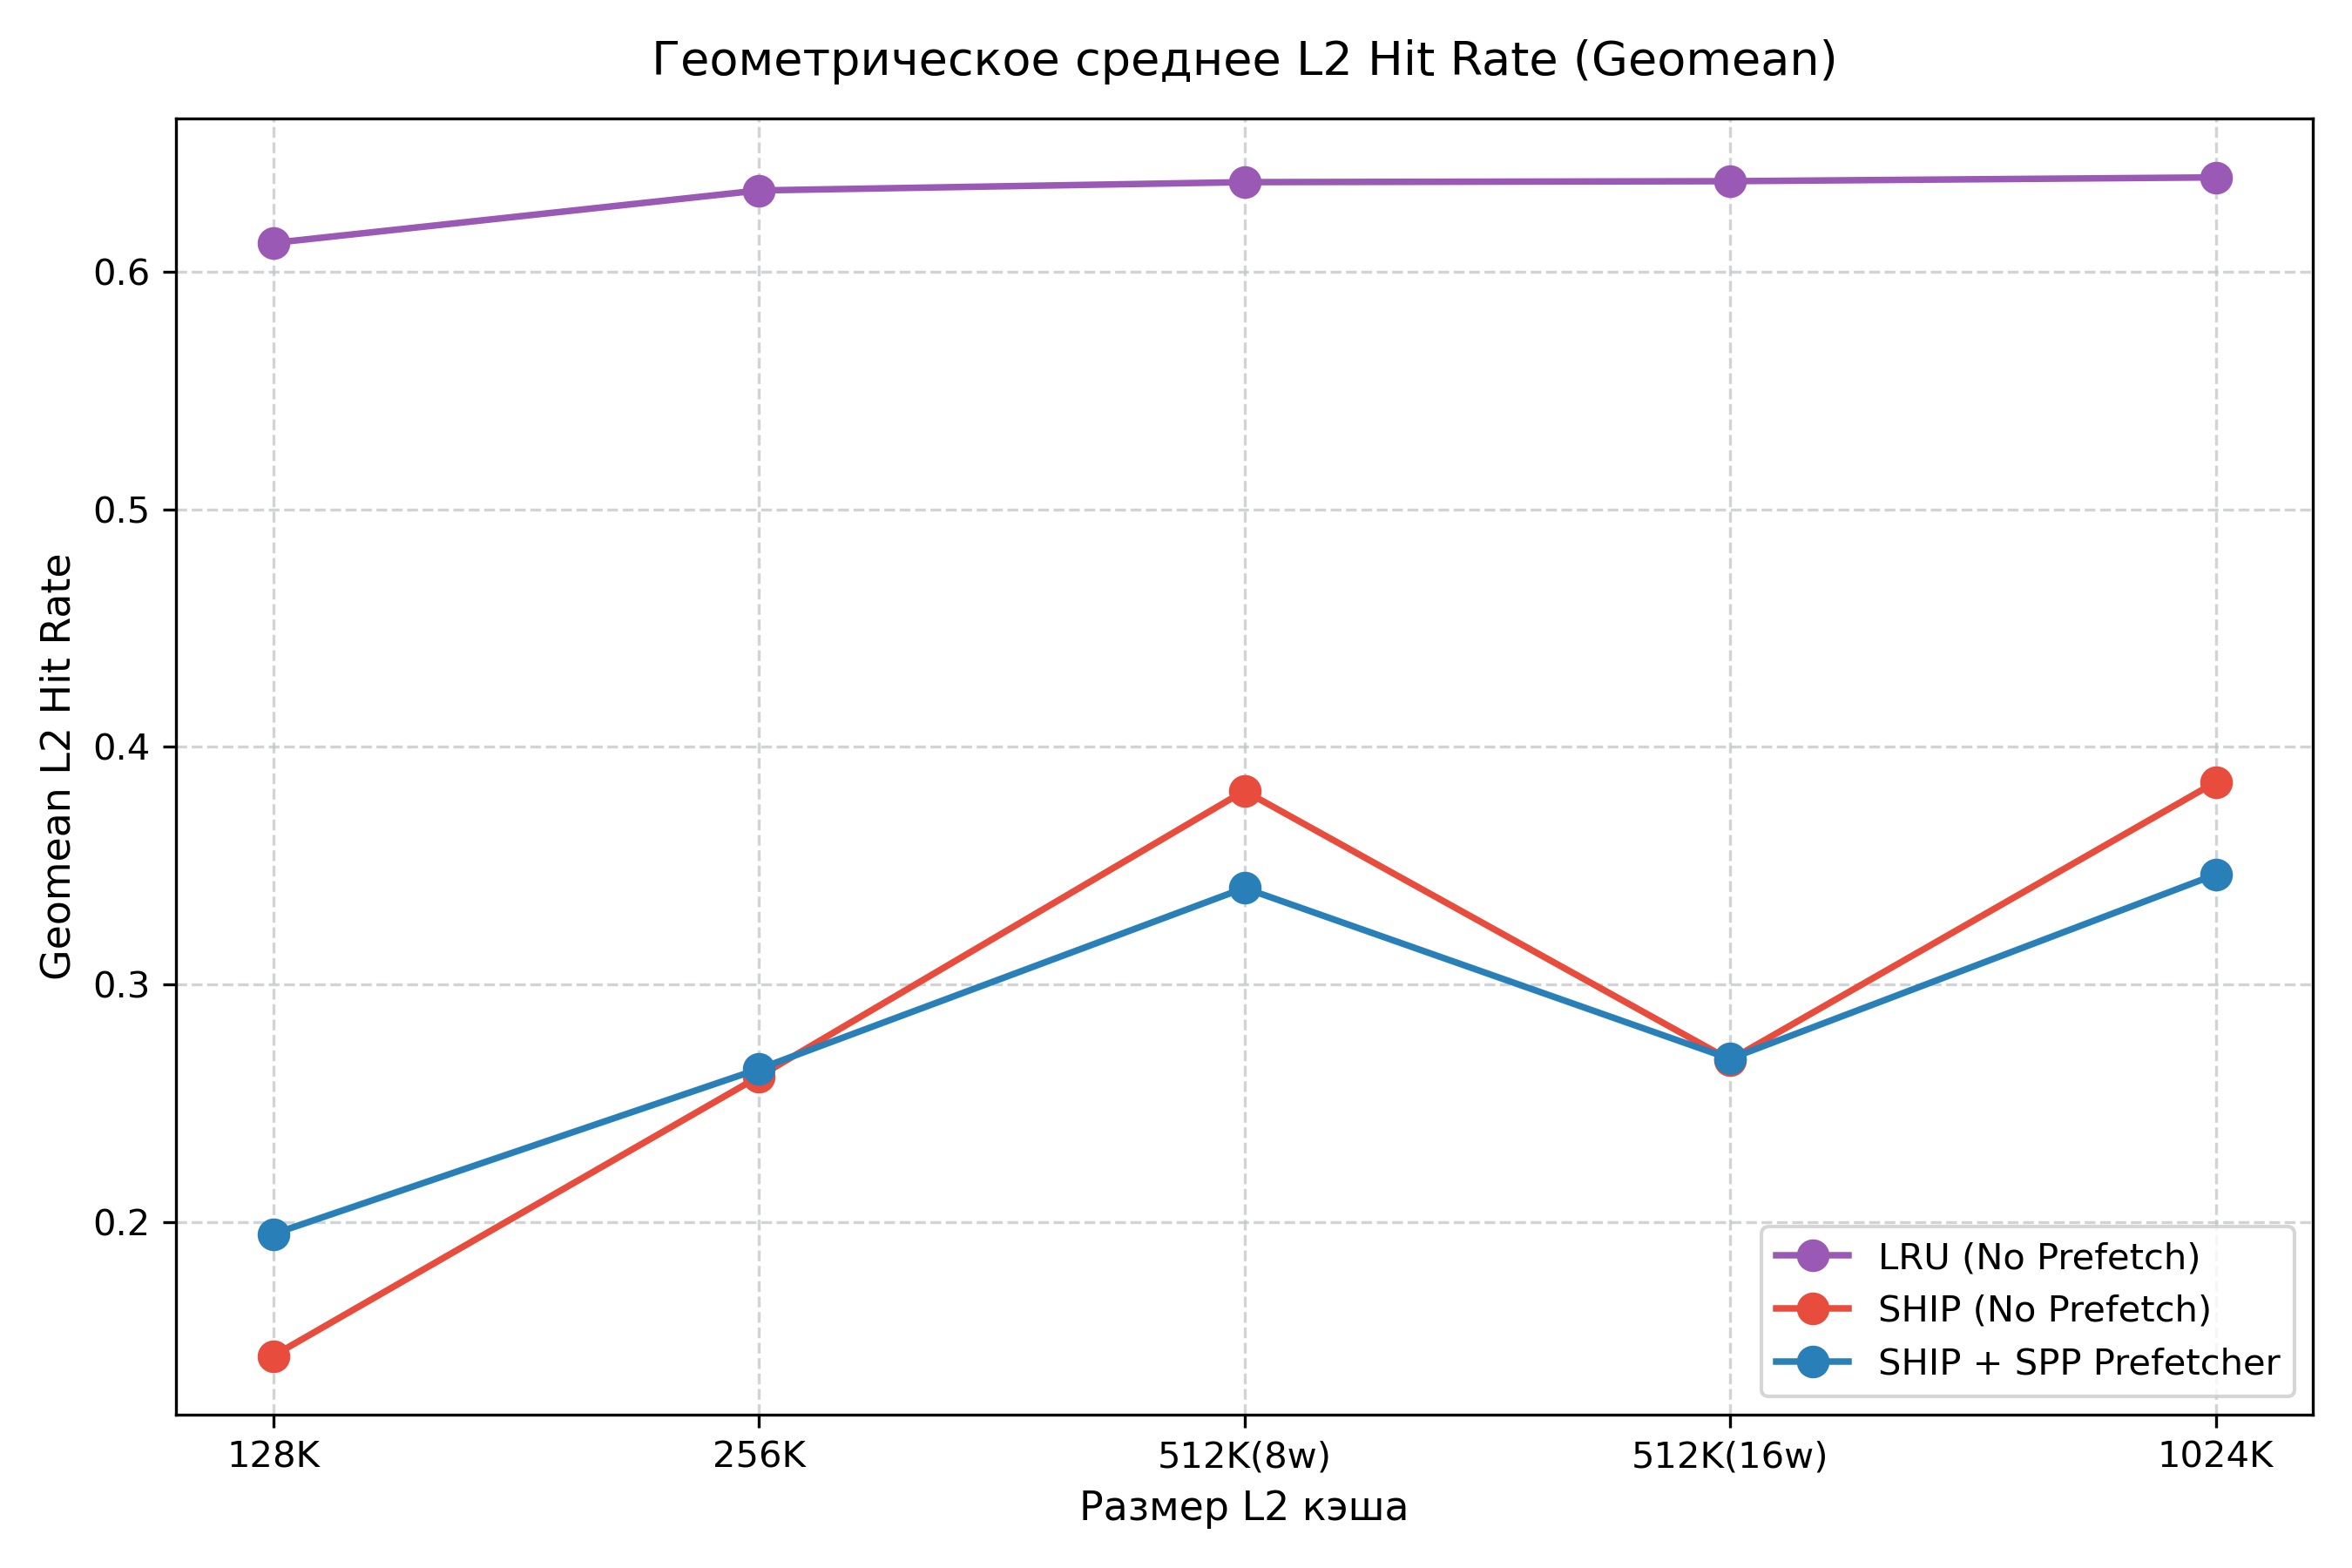
\includegraphics[width=0.8\textwidth]{graph_geomean.png}
    \caption{Зависимость L2 Hit Rate от размера кэша для политик LRU, SHiP и SHiP+SPP.}
    \label{fig:hit_rate}
\end{figure}

\begin{figure}[h!]
    \centering
    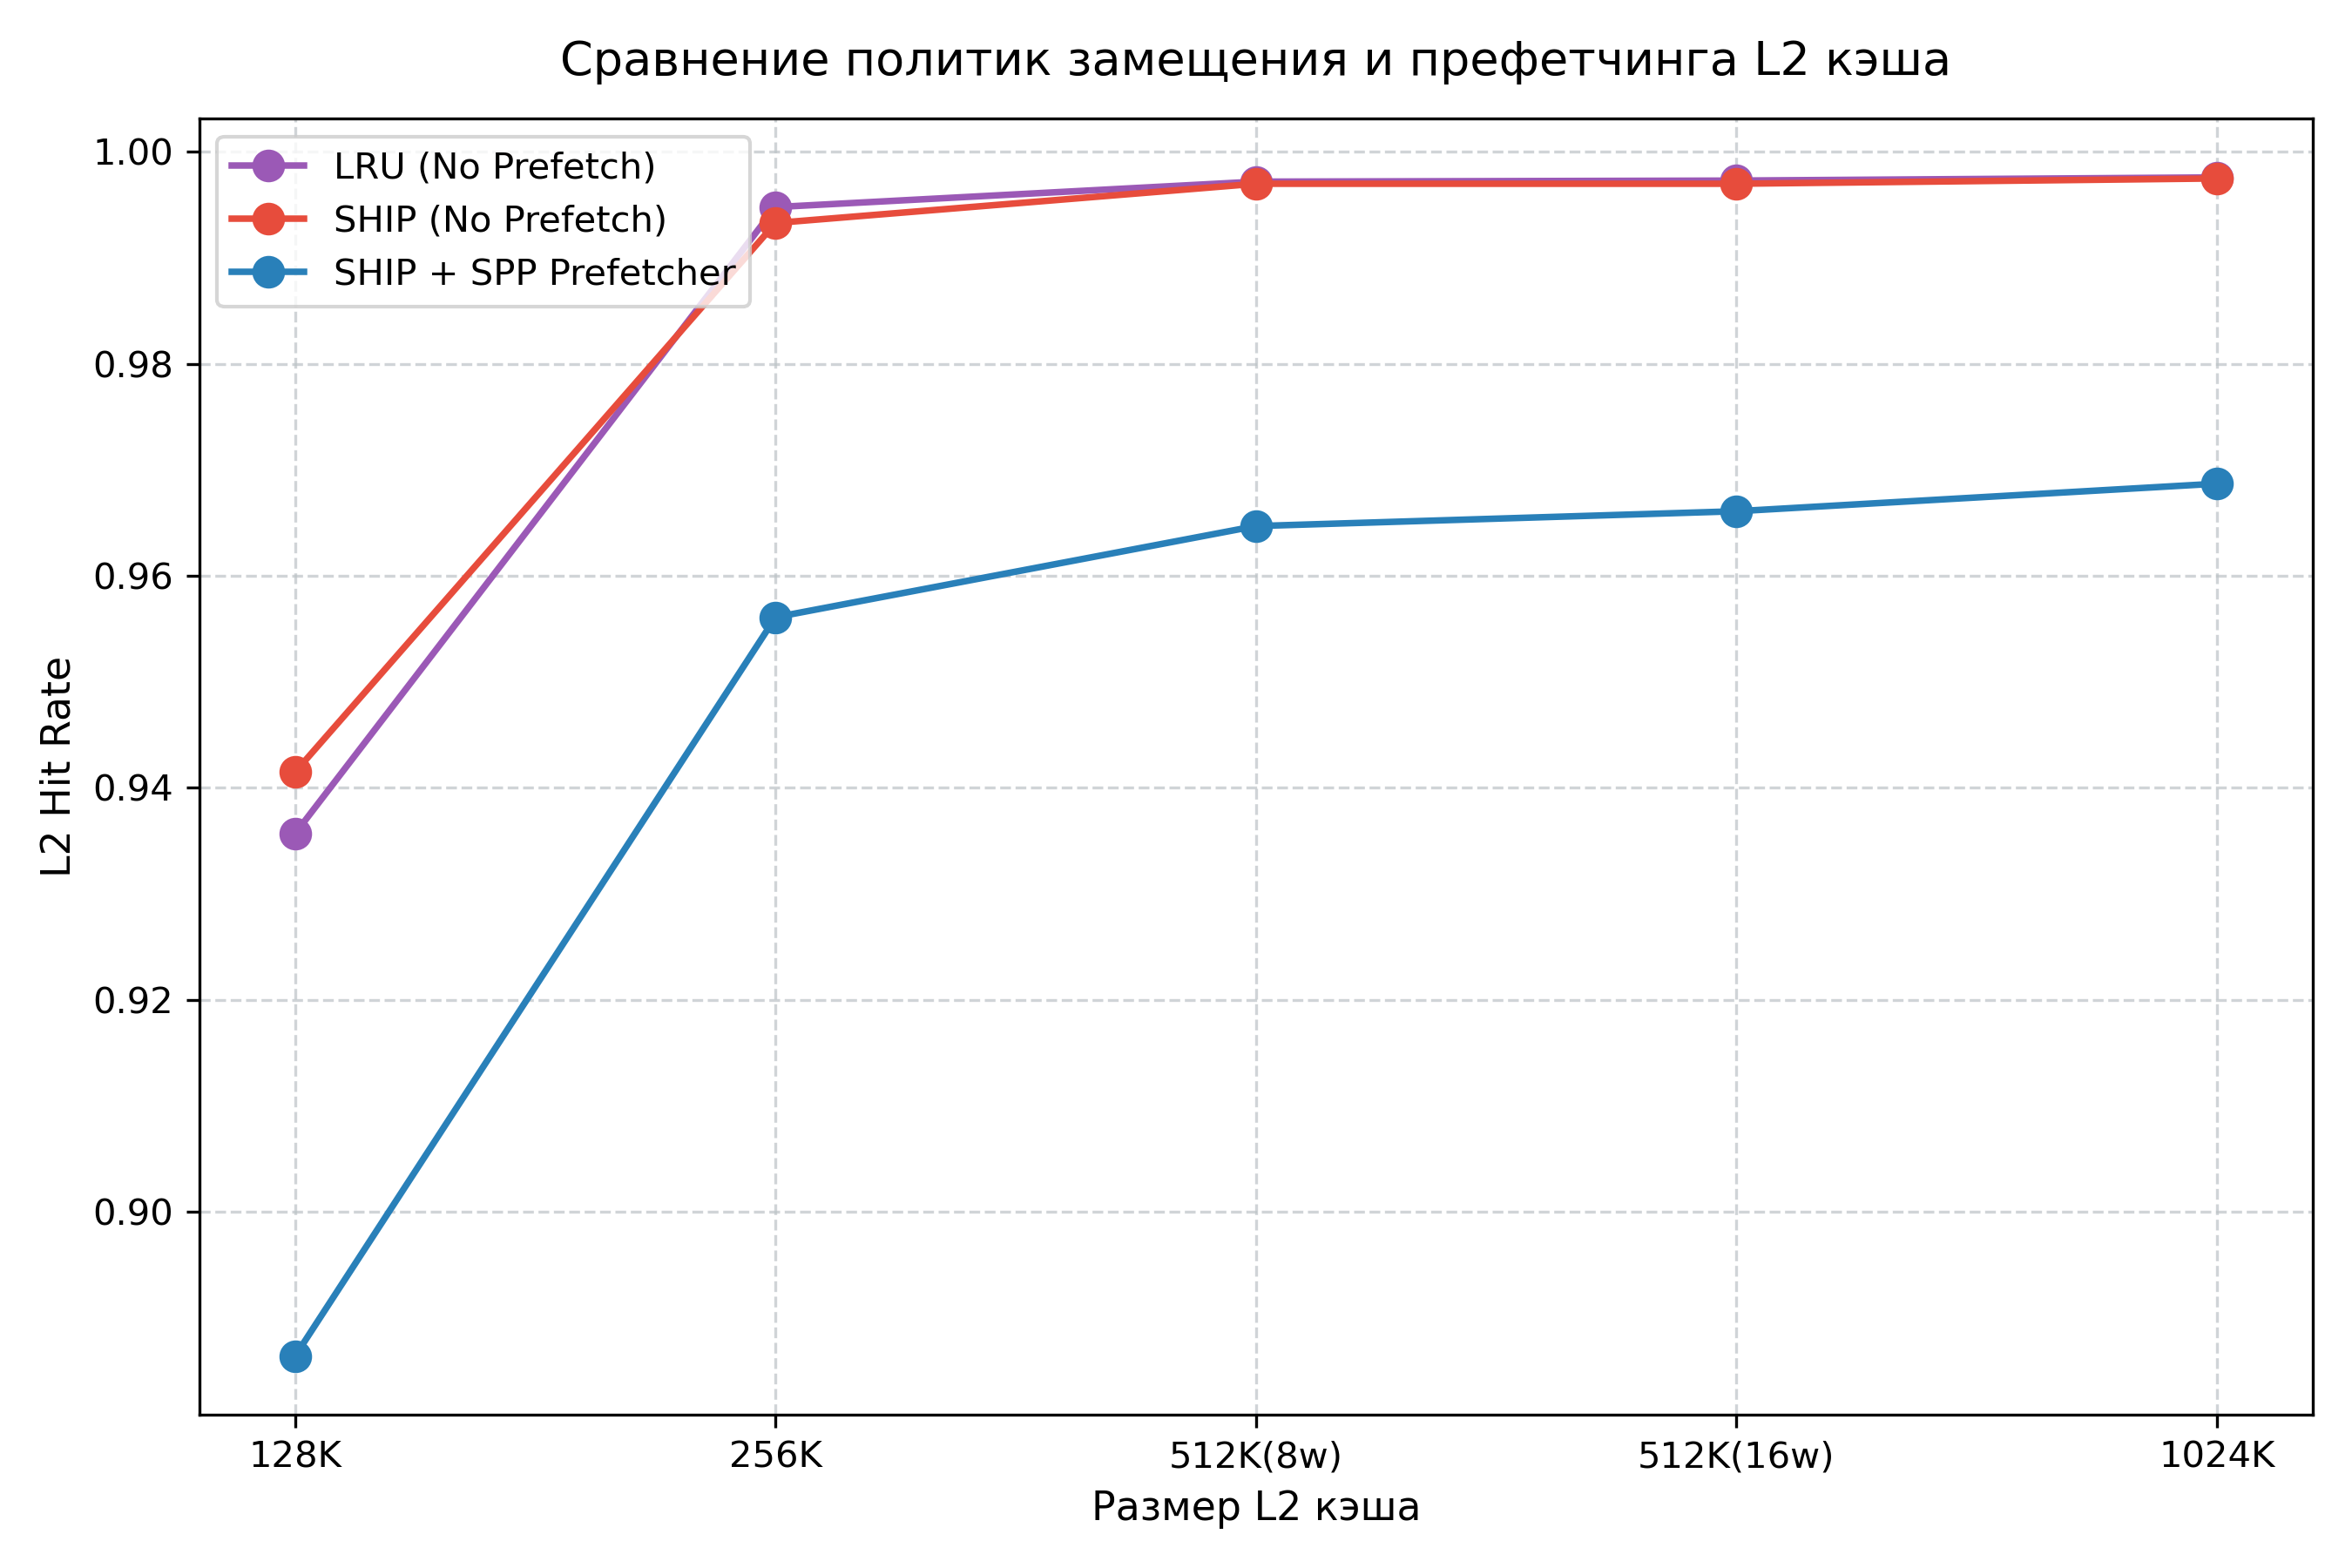
\includegraphics[width=0.8\textwidth]{graph_trace_445_circles.png}
    \caption{Зависимость Hit Rate от размера L2 кэша для трассы 445 (gobmk)}
    \label{fig:res_445}
\end{figure}

\begin{figure}[h!]
    \centering
    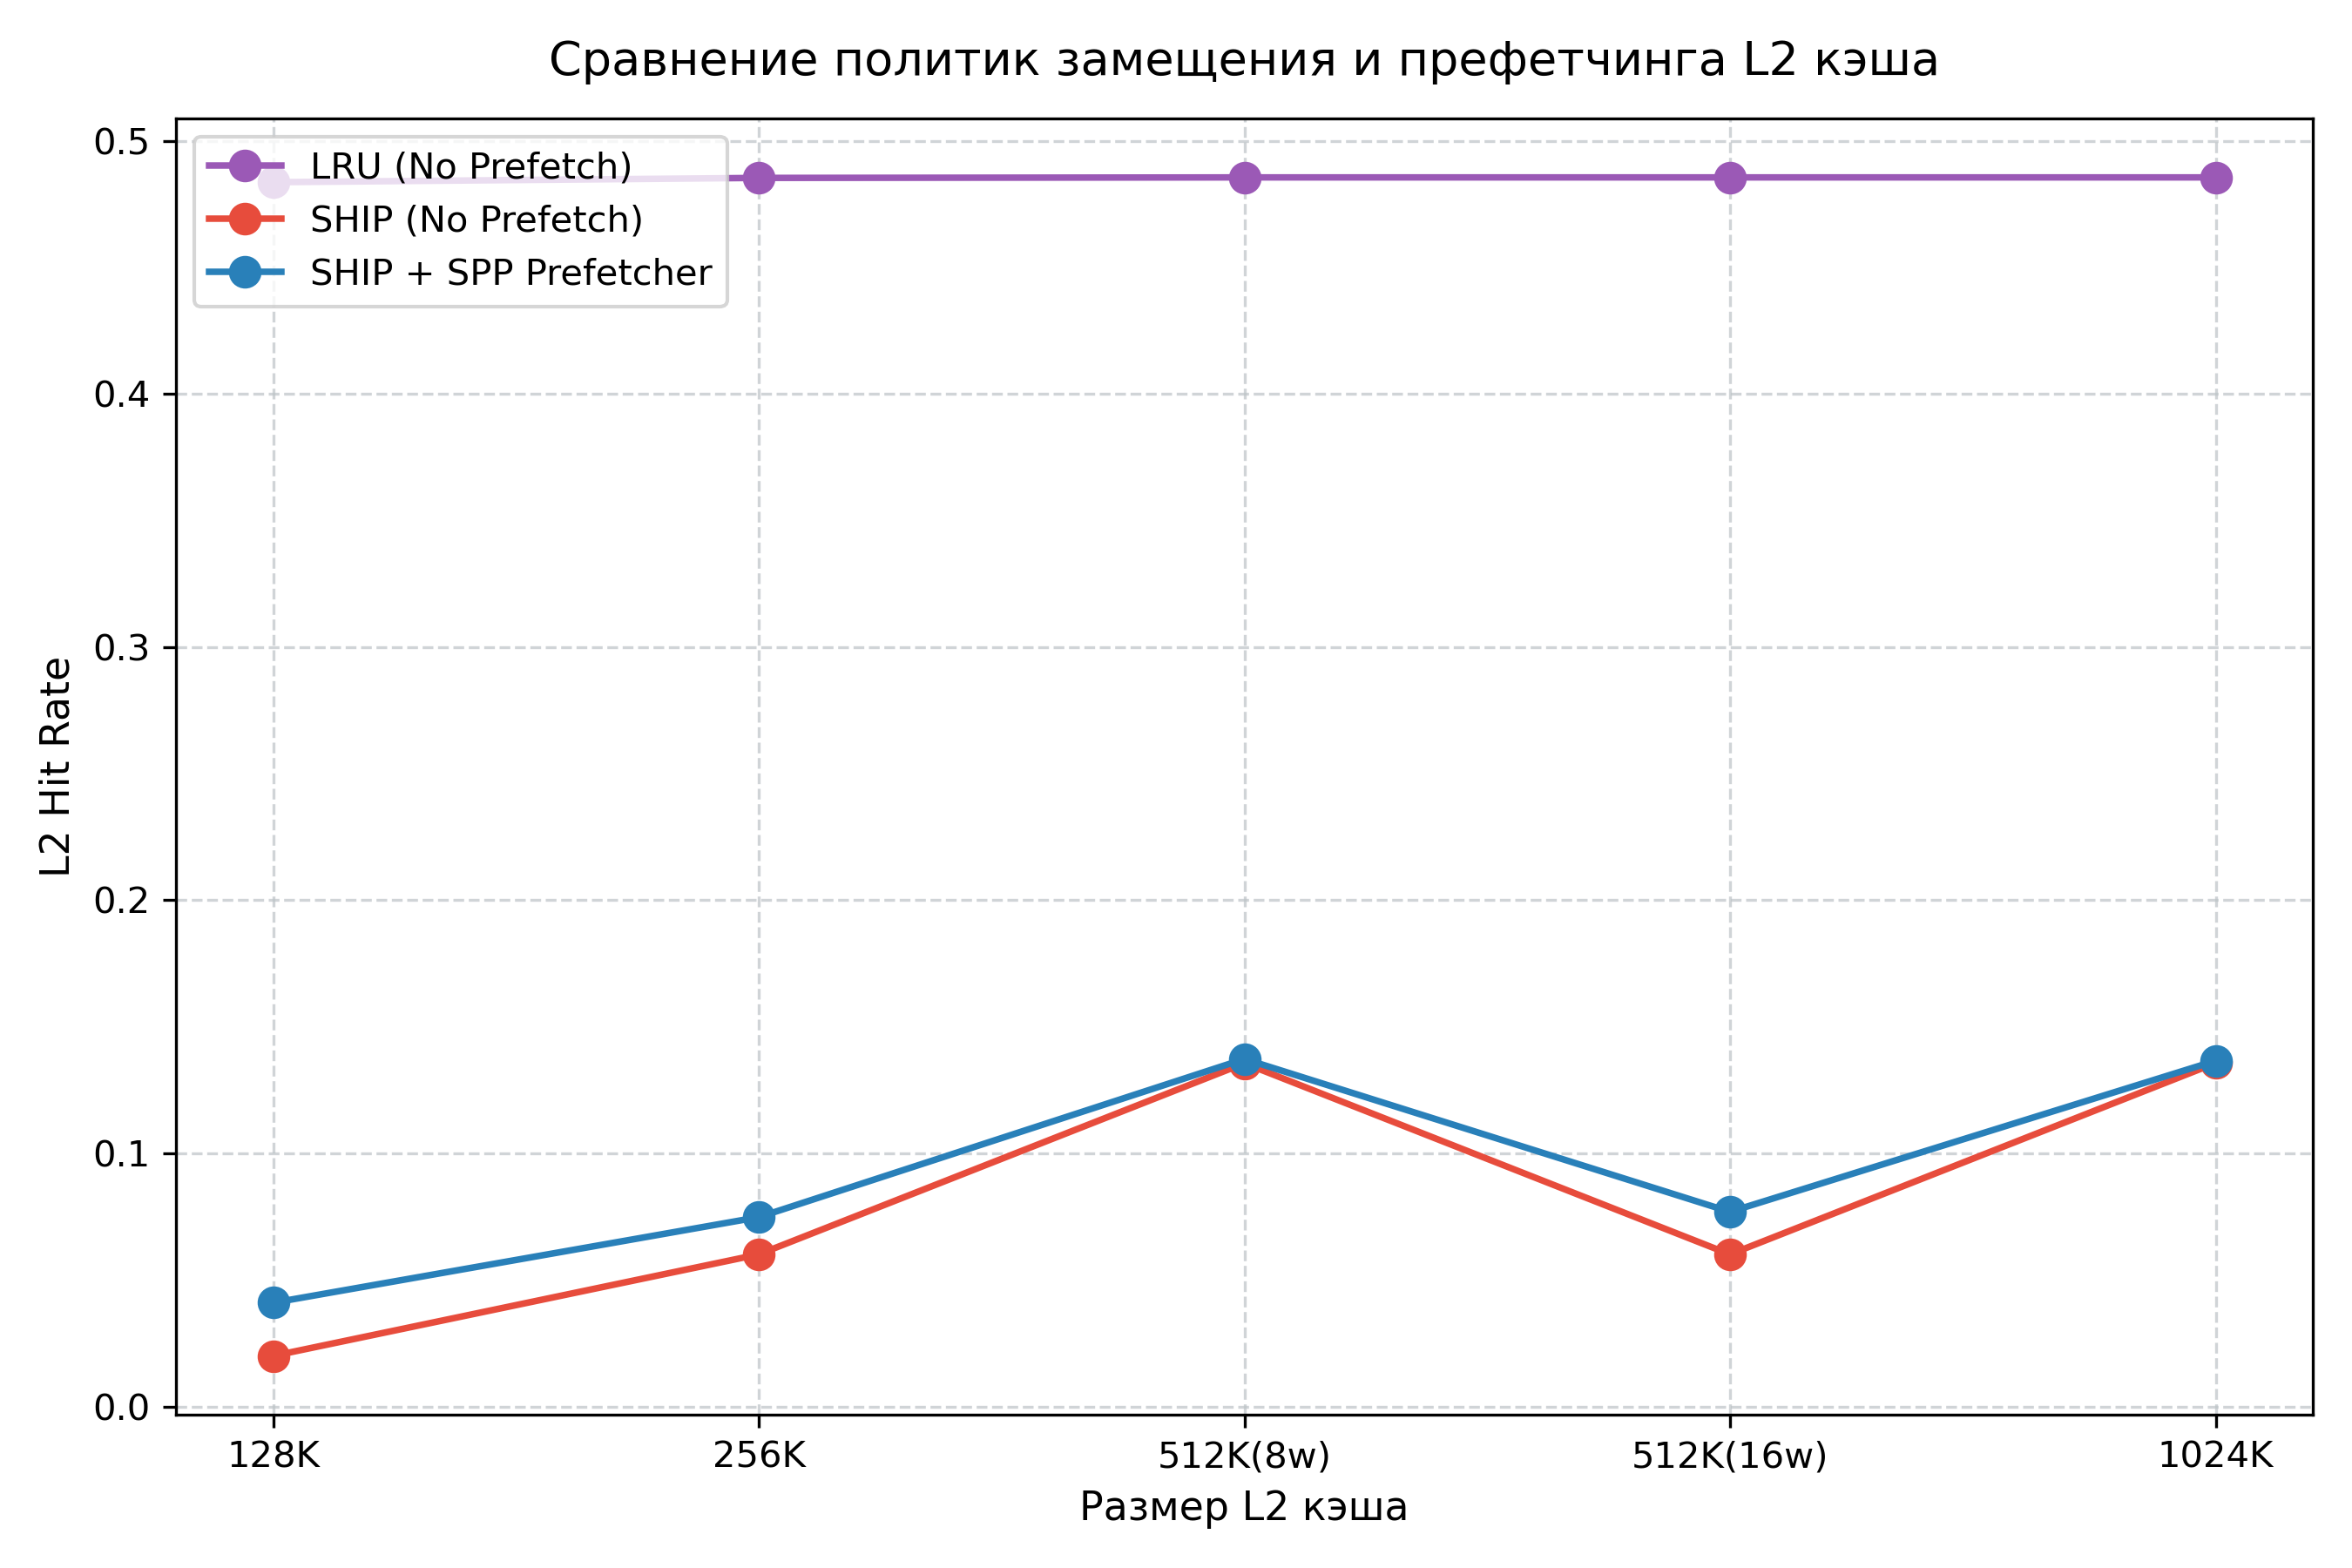
\includegraphics[width=0.8\textwidth]{graph_trace_603_circles.png}
    \caption{Зависимость Hit Rate от размера L2 кэша для трассы 603 (bwaves)}
    \label{fig:res_603}
\end{figure}

\begin{figure}[h!]
    \centering
    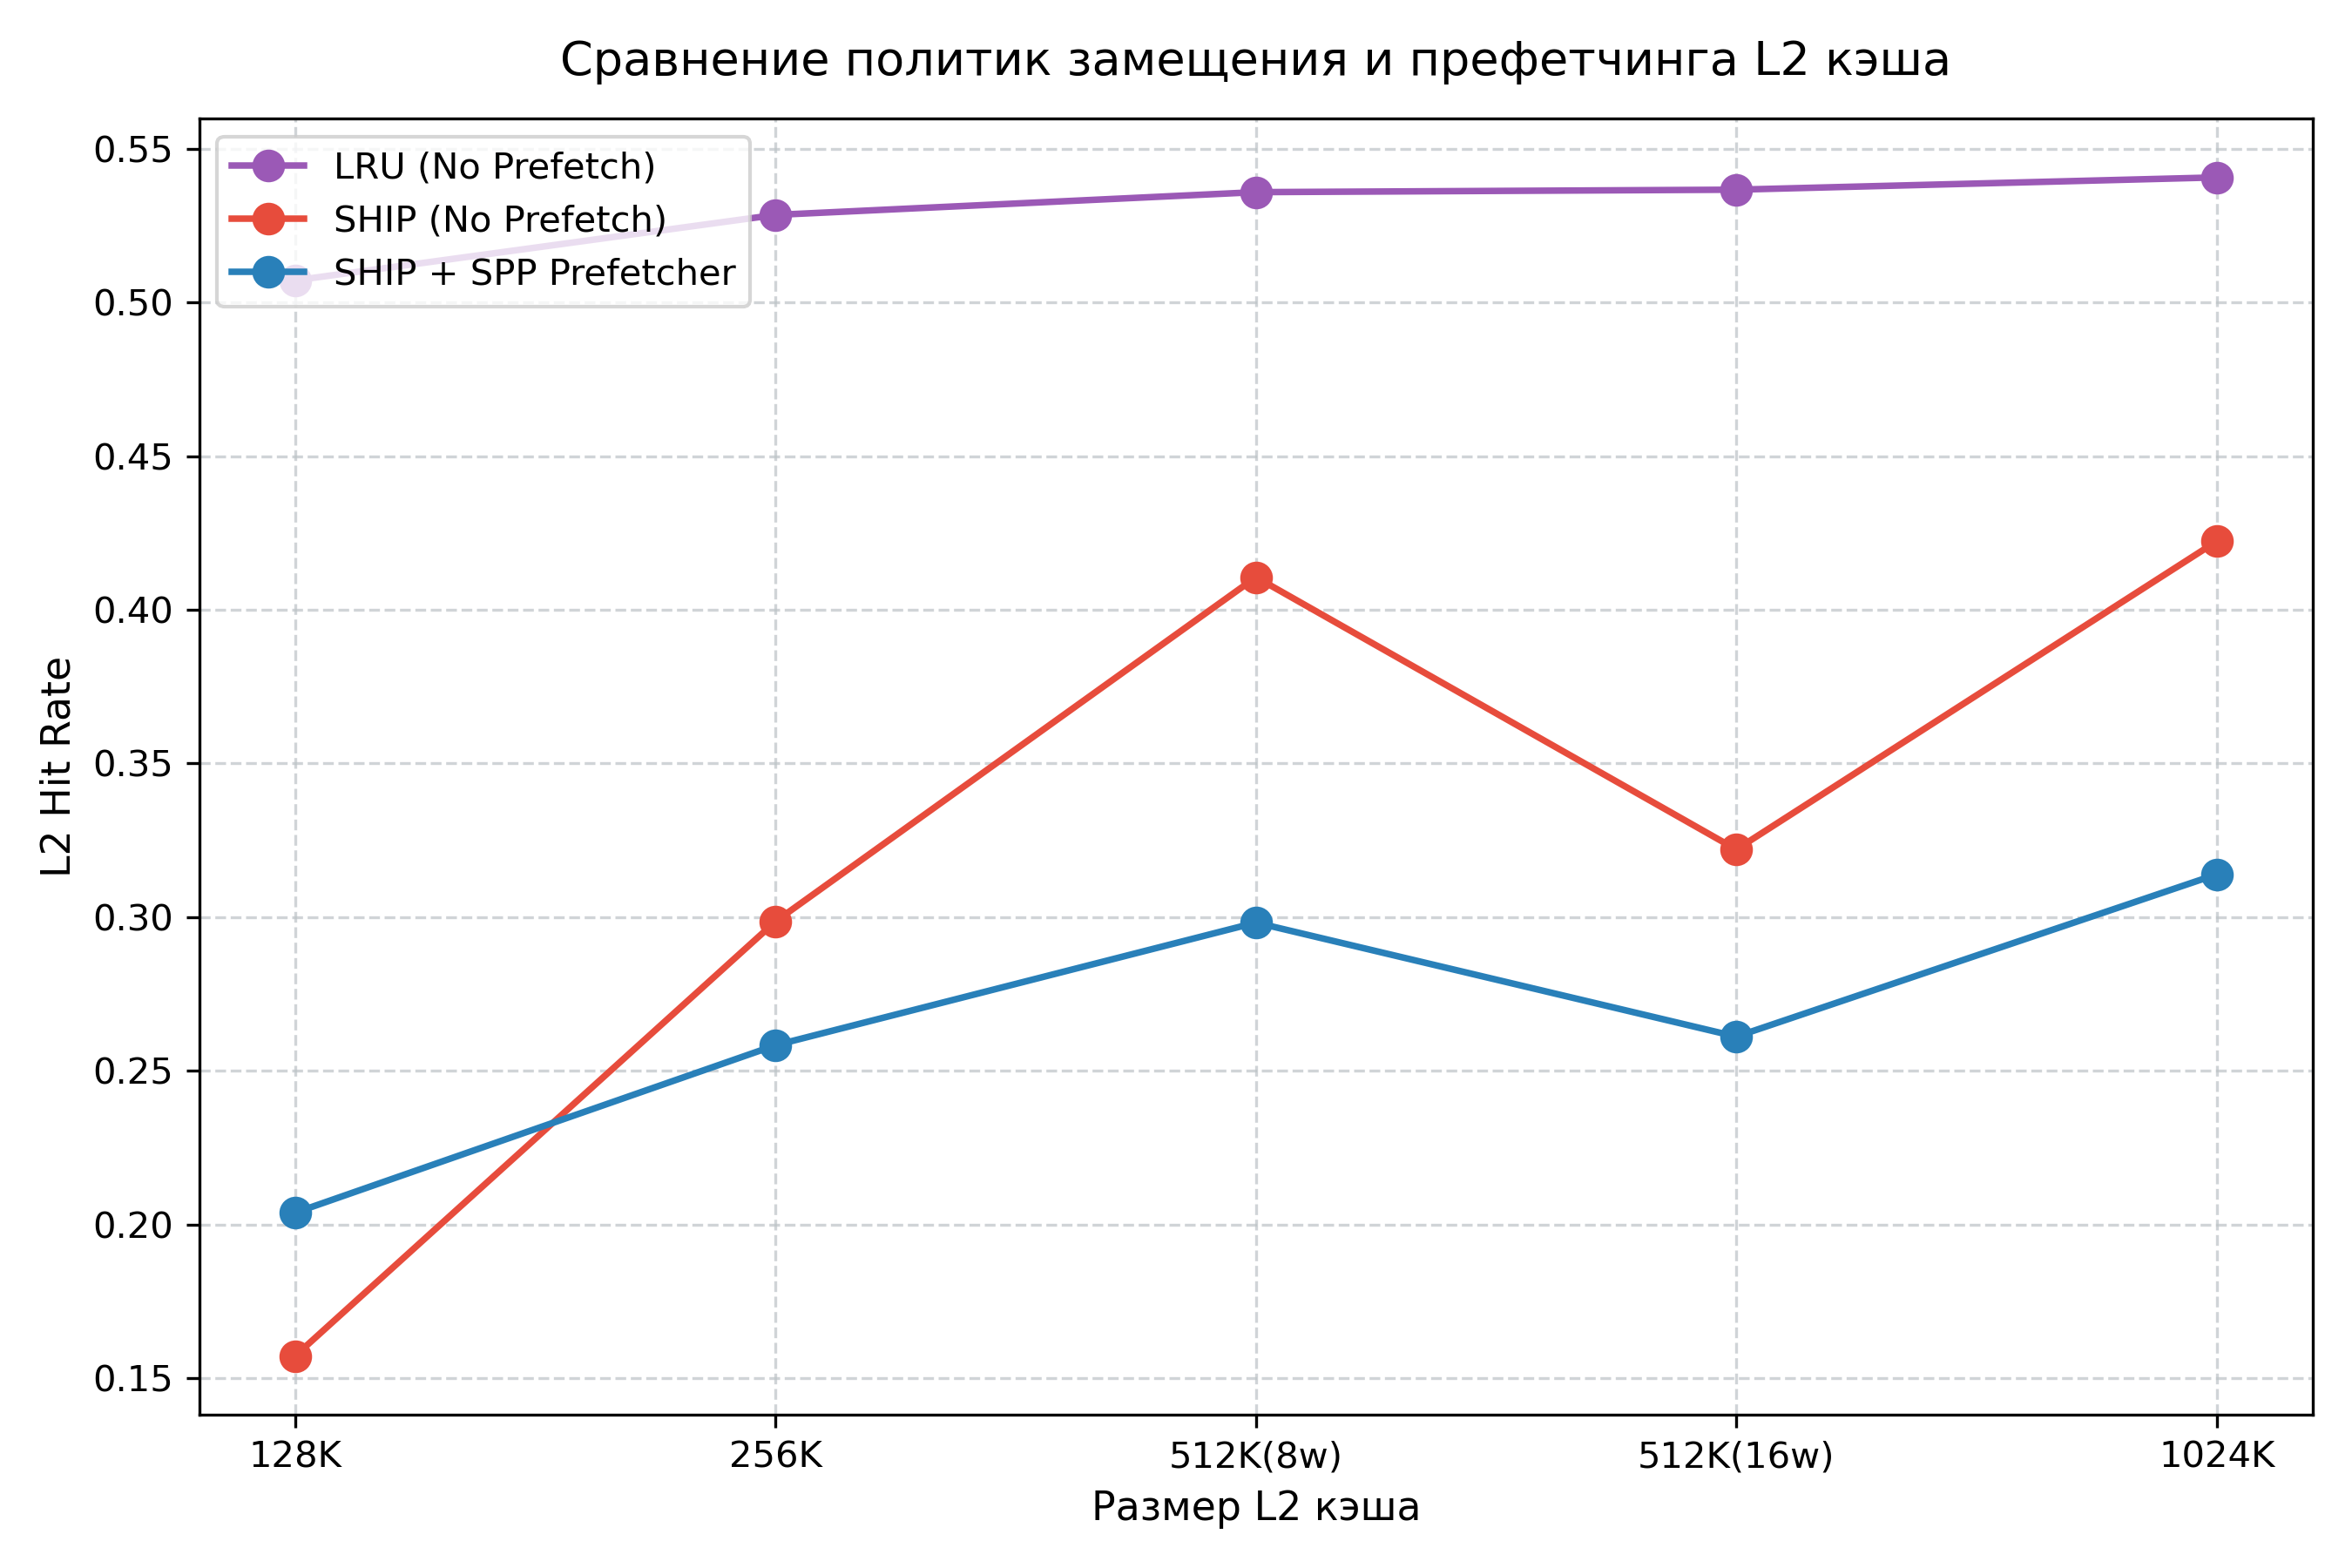
\includegraphics[width=0.8\textwidth]{graph_trace_625_circles.png}
    \caption{Зависимость Hit Rate от размера L2 кэша для трассы 625 (x264)}
    \label{fig:res_625}
\end{figure}

\newpage

\section*{6. Выводы по результатам моделирования}

На основе геометрического среднего L2 Hit Rate по трем трассам сделаны следующие выводы:

\begin{itemize}
    \item \textbf{Влияние политики SHiP:} 
На основе полученных данных можно сделать вывод, что смена политики замещения с LRU на SHIP для данного набора трасс оказалась крайне неудачной. Вместо ожидаемого прироста производительности за счет предсказания с сигнатурами повторного использования данных, SHIP показал деградацию Hit Rate. Возможно повторные обращения происходили слишком поздно, поэтому ship помечал их как ненужные.

\item \textbf{Анализ влияния префетчера SPP на производительность}

Вопреки ожиданиям, на большинстве конфигураций добавление префетчера не только не дало существенного прироста, но и привело к деградации Hit Rate из-за загрязнения кэша. Возможно обращения к данным дыли слишком хаотичными. Так же это могло привести к тому что SPP сбивал с толку SHIP неправильными данными о префетчинге, и SHIP неправильно расставил приоритеты

\begin{itemize}
    \item \textbf{Отрицательный эффект на трассе 445.gobmk:} На данной нагрузке добавление SPP привело к  снижению Hit Rate. В конфигурации 1024K результат упал с 0.9975 (SHIP без префетчера) до 0.9687 (с префетчером). Это свидетельствует о том, что алгоритм SPP генерирует избыточные запросы, которые вытесняют полезные данные из кэша.
    
    \item \textbf{Локальный прирост на малых объемах:} Положительный эффект наблюдается только при минимальных размерах кэша (128K--256K). Например, на трассе 625.x264 при 128K Hit Rate вырос с 0.15 до 0.20. Однако с ростом объема кэша до 1024K этот выигрыш нивелируется, и голый SHIP начинает работать эффективнее.
    
    \item \textbf{603.bwaves:} Для потоковой нагрузки bwaves включение префетчера дает крайне малый прирост на малых объемах (с 0.02 до 0.04), который практически исчезает при достижении объема 512K--1024K.
\begin{itemize}
    \item На объеме 128K зафиксирован небольшой рост Geomean с 0.14 до 0.19.
    \item На объемах 512K и 1024K наблюдается \textbf{падение} показателя с 0.38 до 0.34.
\end{itemize}
\item \textbf{Анализ через среднее геометрическое:}
Агрегированные данные подтверждают, что префетчер SPP оказался скорее вреден:

\end{itemize}


\textbf{Итог:} Включение префетчера SPP оправдано только в условиях жесткого дефицита памяти (128K). В остальных случаях агрессивные предсказания префетчера засоряют кэш данными, которые не используются повторно, что снижает общую эффективность системы.

\item \textbf{Определение оптимального размера кэша}

На основе анализа графиков и средних геометрических показателей можно сделать вывод, что достаточным размером L2 кэша для исследуемого набора трасс является \textbf{512K}. 

\begin{itemize}
    \item Для трассы \texttt{445} точка насыщения достигается уже на \textbf{256K}, после чего Hit Rate стабилизируется на уровне $99.7\%$.
    \item Для трасс \texttt{603} и \texttt{625} значимый прирост наблюдается до отметки \textbf{512K}. Дальнейшее удвоение объема памяти до 1024K дает прирост эффективности менее $1\%$.
\end{itemize}

Таким образом, дальнейшее увеличение объема кэша сверх 512K не приводит к существенному улучшению.

\item \textbf{Что выгоднее увеличивать — значение set или way при равном размере кэша}

При равном объеме кэша 512K сравнение конфигураций 512x16 и 1024x8 показывает следующее:

\begin{itemize}
    \item \textbf{1024 sets, 8-way:} Является более предпочтительной для большинства исследованных трасс. Увеличение количества наборов снижает вероятность коллизий при отображении адресов, в то время как ассоциативности 8-way достаточно для уменьшения конфликтных промахов.
    \item \textbf{512 sets, 16-way:} Высокая ассоциативность не дает значимого прироста Hit Rate (разница менее $0.01\%$), но увеличивает сложность аппаратной реализации и время доступа к данным.
\end{itemize}

Результаты моделирования подтверждают, что избыточная ассоциативность (16-way) может негативно сказываться на точности алгоритмов предикта, таких как SHIP, вызывая деградацию Hit Rate относительно более простых конфигураций.
    
\end{itemize}

\section*{7. Самое интересное задание}

Самыми интересными для меня показались первое и четвёртое задания
\end{document}